\documentclass[a4paper,12pt]{article}

\usepackage{mystyle}

\usepackage{gensymb}
\usepackage{scalerel}
\usepackage{stackengine}


\graphicspath{ {images/} }


% https://tex.stackexchange.com/questions/5461/is-it-possible-to-change-the-size-of-an-arrowhead-in-tikz-pgf
\usetikzlibrary{arrows.meta}


\DeclareMathOperator{\Image}{Im}

\definecolor{pink}{RGB}{218, 3, 174}
\definecolor{violet}{RGB}{148, 0, 211}
\definecolor{green}{RGB}{0, 153, 0}
\definecolor{orange}{RGB}{255, 153, 0}
\definecolor{blue}{RGB}{5, 73, 255}


% https://tex.stackexchange.com/a/101138/135045

\newcommand\widesim[1]{\ThisStyle{%
  \setbox0=\hbox{$\SavedStyle#1$}%
  \stackengine{-.1\LMpt}{$\SavedStyle#1$}{%
    \stretchto{\scaleto{\SavedStyle\mkern.2mu\sim}{.5150\wd0}}{.6\ht0}%
  }{O}{c}{F}{T}{S}%
}}


\newcommand{\BigMiddleThree}{\;\left|\vphantom{\begin{pmatrix} 0\\0\\0 \end{pmatrix}}\right.\;}
\newcommand{\BigMiddleFour}{\;\left|\vphantom{\begin{pmatrix} 0\\0\\0\\0 \end{pmatrix}}\right.\;}


% https://tex.stackexchange.com/questions/63531/how-to-write-quotation-marks-in-math-environment
\DeclareMathSymbol{\mlq}{\mathord}{operators}{``}
\DeclareMathSymbol{\mrq}{\mathord}{operators}{`'}


\DeclareMathOperator{\Imag}{Im}


% https://tex.stackexchange.com/questions/544453/undefined-control-sequence-after-paragraph
\renewcommand{\paragraph}[1]{\noindent\textbf{#1}\quad}


% https://tex.stackexchange.com/questions/36851/skipping-line-after-proof-in-proof-environment#comment73553_36851
\newcommand{\proofindent}{\hspace*{\fill}\par\vspace{0.5em}\noindent}


% https://tex.stackexchange.com/questions/4813/extendible-equals-sign
\makeatletter
\newcommand*{\Relbarfill@}{\arrowfill@\Relbar\Relbar\Relbar}
\newcommand*{\xeq}[2][]{\ext@arrow 0055\Relbarfill@{#1}{#2}}
\makeatother


% https://tex.stackexchange.com/questions/279100/typeset-the-shrug-%C2%AF-%E3%83%84-%C2%AF-emoji
\newcommand{\shrug}[1][]{%
\begin{tikzpicture}[baseline,x=0.8\ht\strutbox,y=0.8\ht\strutbox,line width=0.125ex,#1]
  \def\arm{(-2.5,0.95) to (-2,0.95) (-1.9,1) to (-1.5,0) (-1.35,0) to (-0.8,0)};
  \draw \arm;
  \draw[xscale=-1] \arm;
  \def\headpart{(0.6,0) arc[start angle=-40, end angle=40,x radius=0.6,y radius=0.8]};
  \draw \headpart;
  \draw[xscale=-1] \headpart;
  \def\eye{(-0.075,0.15) .. controls (0.02,0) .. (0.075,-0.15)};
  \draw[shift={(-0.3,0.8)}] \eye;
  \draw[shift={(0,0.85)}] \eye;
  % draw mouth
  \draw (-0.1,0.2) to [out=15,in=-100] (0.4,0.95); 
\end{tikzpicture}}



% https://tex.stackexchange.com/a/314638/135045
\newcommand{\diff}{\mathop{}\!d\!}


% https://tex.stackexchange.com/a/22134/135045
\newcommand{\widebar}[1]{\overline{#1\mkern-1.5mu}\mkern 1.5mu}  % Needed to remove mkern trick from left side (otherwise looked not so good)




\author{Алексеев Василий}


\title{Семинар 2}
\date{9 сентября 2024}


\begin{document}
  \maketitle
  
  \tableofcontents

  \thispagestyle{empty}
  
  \newpage
  
  
  
  \vspace*{\fill}
  
  \noindent
  \emph{
    К формулировкам и доказательствам (если такие вообще приводятся) стоит относиться критически.
    Основное в этом конспекте~---~решение задач (но ``критичность'' и здесь лучше не отключать).
    За строгой, ясной и последовательной теорией лучше обращаться к ``нормальным'' источникам.
    (Например, к лекциям.)
  }
  
  \vspace*{\fill}
  
  \thispagestyle{empty}
  
  \newpage
  
  
  \pagenumbering{arabic}


  \section{Числа (продолжение)}
    
  Множество $X \hm\subseteq$ называется \emph{ограниченным}, если оно ``ограничено'' (с двух сторон на числовой прямой):
  \begin{equation}\label{eq:bounded-set}
    \exists C \in \RR\colon \forall x \in X \to {-}C < x < C\quad (\mbox{или}\ |x| < C, \mbox{или даже}\ |x| \leq C)
  \end{equation}
  
  Также говорят ещё о, например, \emph{ограниченном сверху} множестве~$X$~---~таком множестве, которое ограничено ``справа'' на числовой прямой:
  \[
    \exists C \in \RR\colon \forall x \in X \to x < C\quad (\mbox{или}\ x \leq C)
  \]
  При этом число $C$, такое что $x \hm\leq C\ \forall x \hm\in X$ (``правая граница'') называется \emph{верхней гранью} множества~$X$.\footnote{В определении верхней границы уже важно, чтоб неравенство $x \hm\leq C$ было нестрогое, потому что допускается, чтоб сама верхняя граница также была элементом множества $X$.}
  
  Аналогично определяются \emph{ограниченное снизу} множество и \emph{нижняя грань} множества.
  
  \begin{figure}[ht]
    \centering
    \includegraphics[width=0.6\linewidth]{images/sup-inf}
    
    \caption{
      Ограниченное (с двух сторон) множество $X \hm\subset \RR$ и его точная верхняя~$\sup X$ и нижняя~$\inf X$ грани.
    }
    \label{fig:sup-inf}
  \end{figure}
  
  Очевидно, верхняя грань~---~если есть хотя бы одна, то она не одна~(\ref{fig:sup-inf}).
  (Любое число, большее уже найденной верхней грани, также будет верхней гранью.)
  Поэтому имеет смысл говорить о самой маленькой (самой ``плотно прилегающей'' к~$X$) верхней грани~---~\emph{точной верхней грани}.
  Таким образом, число~$C \hm\in \RR$ называется точной верхней гранью множества~$X$, если:
  \begin{enumerate}
    \item оно само является верхней гранью~$X$:
      \[
        \forall x \in X \to x \leq C
      \]
    \item оно является самой маленькой верхней гранью (нет верхней грани меньше):
      \[
        \forall C' < C\ \exists x \in X\colon x > C'
      \]
  \end{enumerate}
  
  % TODO: про расширенную числовую прямую
  
  \begin{example}
    Рассмотрим множество
    \[
      X \hm= \left\{\frac{1}{n} \mid n \in \NN \right\} = \left\{1, \frac{1}{2}, \frac{1}{3}, \ldots\right\}
    \]
    Кажется, что точной нижней гранью будет число~$0$.
    Покажем это.
    
    Так, $0$ в самом деле нижняя грань: $\frac{1}{n} \hm\geq 0$ $\forall n \hm\in \NN$.
    Но нет ли ещё чего-то ``после'' нуля, что бы тоже было нижней гранью (нет ли ``зазора'' между~$0$ и $X$)?
    Допустим, найдётся число $L \hm> 0$ (очевидно, также $L \hm< 1$), которое тоже будет верхней гранью.
    Но тогда можно будет найти элемент $x_0 \hm= \frac{1}{n_0}$ из~$X$, который окажется меньше:
    \[
      \frac{1}{n_0} < L \leftrightarrow n_0 > \frac{1}{L} \Rightarrow n_0 = \left\lceil\frac{1}{L}\right\rceil + 1
    \]
    (где ${} + 1$ справа~---~``на всякий случай'', если вдруг получится, что $\frac{1}{L}$ уже само целое).
    
    Значит, не существует нижней грани больше~$0$, то есть~$0$ есть точная нижняя грань.
  \end{example}
  
  
  \section{Последовательности}
  
  Последовательностью~$\{x_n\}$ называется занумерованная ($n \hm\in \NN$) совокупность бесконечного числа элементов~$x_n$ одной природы (чисел, в случае числовой последовательности).
  Так как элементов в последовательности бесконечно много, то просто взять и все перечислить их нельзя, и нужно какое-то \emph{правило}, по которому можно определить член последовательности~$x_n$ с заданным номером~$n$.
  Таким образом, о последовательности можно думать как о \emph{функции}~$f$, осуществляющей сопоставление между множеством номеров~$\NN$ и множеством чисел (например, $\RR$):
  \[
    %\begin{aligned}
      %&f\colon \NN \to \RR\\
      %&\NN \ni n \overset{f}{\mapsto} x_n \in \RR
    %\end{aligned}
    \NN \ni n \overset{f}{\mapsto} x_n \in \RR
  \]
  
  \begin{example}
    Можно взять последовательность из натуральных чисел~(\ref{fig:sequence-examples}):
    \begin{equation}\label{eq:nat-seq}
      \begin{aligned}
        &\{1, 2, 3, \ldots\}\\
        &x_1 = 1,\ x_2 = 2,\ x_3 = 3,\ \ldots\\
        &x_n = n
      \end{aligned}
    \end{equation}
    
    Из чисел, обратных натуральным:
    \begin{equation}\label{eq:1-div-nat-seq}
      \left\{1, \frac{1}{2}, \frac{1}{3}, \ldots\right\} = \left\{\frac{1}{n}\right\}
    \end{equation}
    
    \begin{figure}[ht]
      \centering
      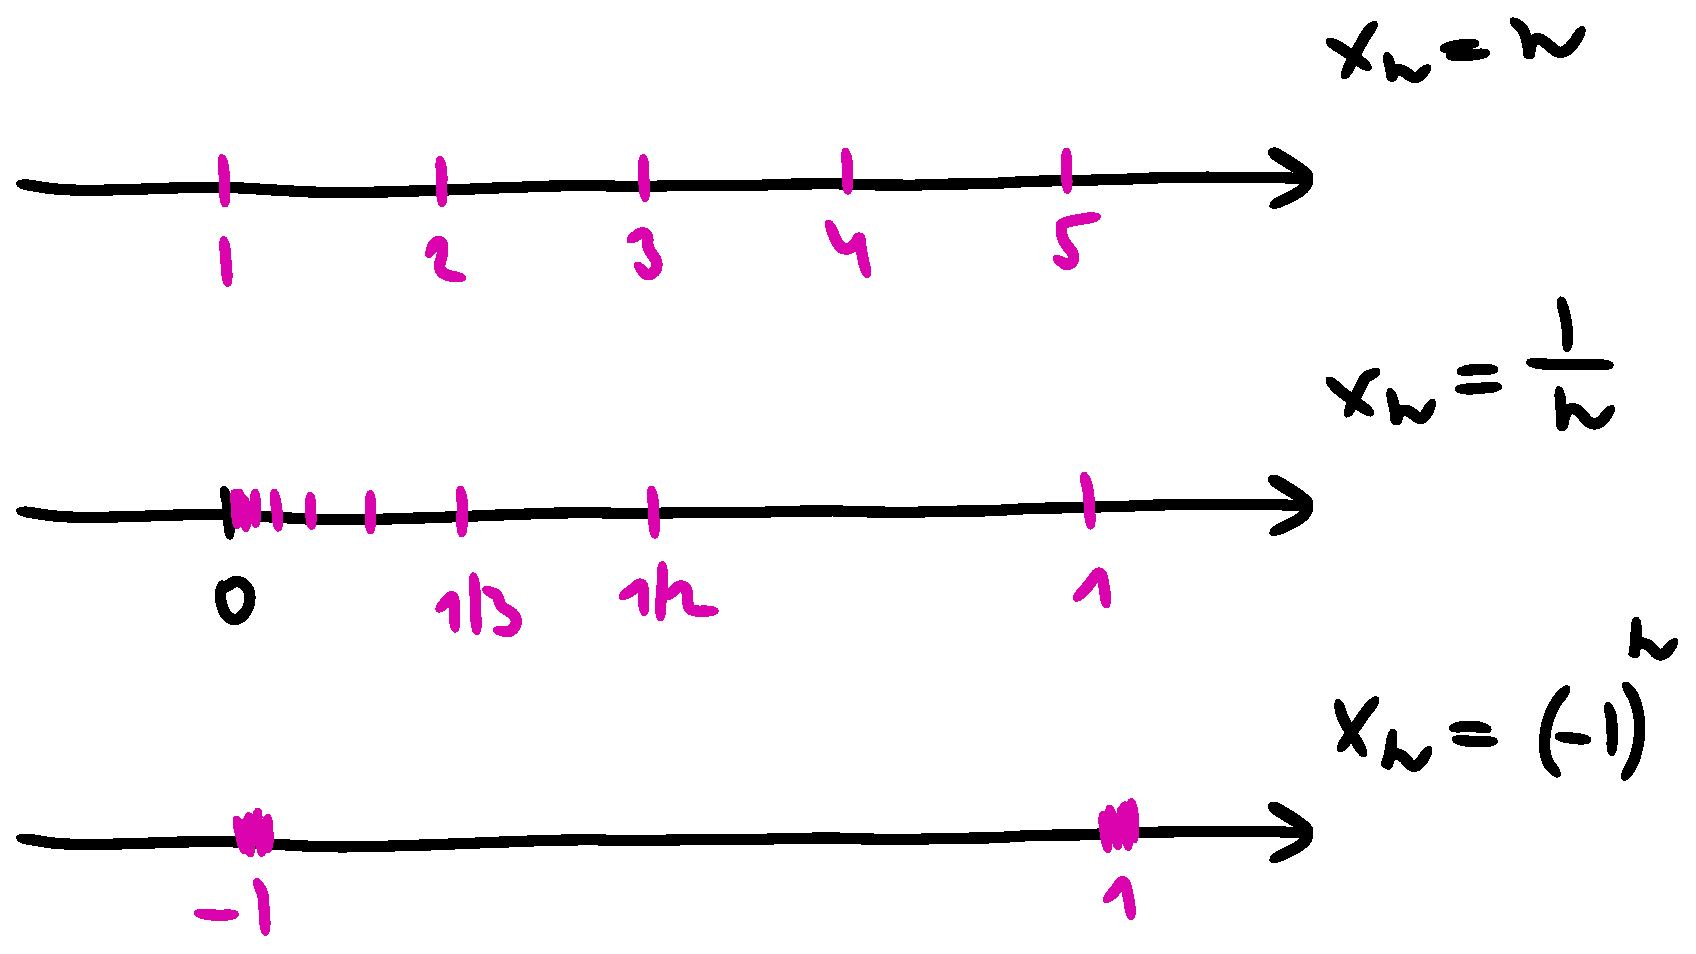
\includegraphics[width=0.8\linewidth]{images/sequence-examples}
      
      \caption{
        Примеры последовательностей.
      }
      \label{fig:sequence-examples}
    \end{figure}
    
    Не обязательно, чтобы все элементы последовательности были различными (элементы могут повторяться~---~\emph{номера} у них будут разные).
    Например, последовательность из двух различных чисел:
    \begin{equation}\label{eq:1-pow-minus-1}
      \{+1, -1, +1, -1, \ldots\} = \left\{(-1)^{n + 1}\right\}
    \end{equation}
    или последовательность из одного числа: $\{1, 1, 1, \ldots\}$.
  \end{example}
    
  Кроме ``уникальности'' элементов, последовательности характеризуются ещё тем, что могут быть \emph{ограниченными} (например,~\eqref{eq:1-pow-minus-1} или~\eqref{eq:1-div-nat-seq}) и \emph{неограниченными} (например,~\eqref{eq:nat-seq}).
  Ограниченность последовательности означает то же самое, что и ограниченность множества~\eqref{eq:bounded-set}:\footnote{
    Хотя последовательность и не множество.
    Скорее, ограниченность последовательности как функции~$f\colon \NN \hm\to \RR$ равносильна ограниченности \emph{множества значений} этой функции $E_f \hm= f(\NN) \hm= \Imag f \hm\equiv \{f(n) \hm\mid n \hm\in \NN\}$.
  }
  последовательность~$\{x_n\}$ ограничена, если найдётся $C \hm> 0$, такое что $|x_n| \hm< C$, $\forall n \hm\in \NN$.
  
  Последовательность~---~это не только элементы, но ещё и порядок этих элементов.
  Поэтому отличительной чертой последовательности может быть какое-нибудь ``особенное'' расположение элементов друг относительно друга, расположение их на числовой прямой.
  Так, элементы~\eqref{eq:1-pow-minus-1} ``скачут'' туда-сюда.
  В отличие от элементов~\eqref{eq:nat-seq}, которые идут по возрастанию (слева направо по числовой прямой), или элементов~\eqref{eq:1-div-nat-seq}, идущих по убыванию~---~такие последовательности называются \emph{монотонными}.
  Более того, можно рассмотреть последовательность, например:
  \[
    \{404, 1, 2, 3, \ldots\},\quad x_n = \left\{
      \begin{aligned}
        &404, & &\mbox{если}\ n = 1\\
        &n - 1, & &\mbox{если}\ n \geq 2
      \end{aligned}
    \right.
  \]
  Которая, строго говоря, не является возрастающей (потому что в начале последовательности происходит что-то ``не то'').
  Но с какого-то момента (с какого-то номера) всё становится ``ровно'', члены начинают идти от меньшего к большему.
  Так как последовательности бесконечны по числу элементов, то особенно интересно их поведение ``в пределе'': если в начале наблюдается какая-то ``утряска'' (случайный порядок элементов), а с какого-то момента до бесконечности всё ``хорошо'' (становится монотонной), то и всю последовательность в целом можно считать монотонной.
  Точнее~---~монотонной с некоторого номера.
  Итак, последовательность~$\{x_n\}$ монотонно возрастает (начиная с номера $N \hm\in \NN$), если
  \[
    x_{n + 1} \geq x_n,\quad \hphantom{n \geq {}} n \geq N
  \]
  или, что то же самое:
  \[
    x_n \geq x_k,\quad n \geq k \geq N
  \]
  Говорят, что последовательность \emph{строго} возрастает, если знак неравенства строгий: $x_{n + 1} \hm> x_n$.
  
  Что ещё может быть ``интересного'' в расположении элементов последовательности?
  Возьмём, к примеру, последовательности натуральных чисел~\eqref{eq:nat-seq} и ``плюс-минус один''~\eqref{eq:1-pow-minus-1}.
  У второй, в отличие от первой, есть две точки~---~$\pm 1$,~---~около которых ``сконцентрировано'' бесконечное число элементов последовательности.
  У последовательности чисел, обратных натуральным~\eqref{eq:1-div-nat-seq} тоже есть ``точка притяжения'' (но уже единственная): её элементы всё ближе подходят к нулю по мере увеличения номера.
  А у последовательности, например
  \[
    \{0, 1, 0, 2, 0, 3, \ldots\}
  \]
  точка притяжения есть (рядом с ней лежит бесконечное число элементов)~---~точка ноль~---~тоже единственная, но при этом также бесконечное число элементов лежит не рядом с ней, а ``где-то ещё''.
  (При этом, в отличие от~\eqref{eq:1-div-nat-seq}, ноль является ещё и членом последовательности.)
  Получается, часть элементов последовательности ``притянулись'', часть нет.
  Такие точки, к которым всё ближе и ближе ``подбирается'' бесконечное количество членов последовательности, называются \emph{частичными пределами}.
  И это настолько важная тема, что про неё будет отдельно далее в разделе~(\ref{seq:limit}).
  
  Из сюжета выше видно, что бывает смысл из всей последовательности $\{x_n\}_{n = 1}^{\infty}$ выделять... \emph{подпоследовательность}~---~бесконечную по числу совокупность элементов, объединённых как бы в новую последовательность~$\{x_{n_k}\}_{k = 1}^{\infty}$, в том же порядке, как они были расположены в исходной последовательности: $n_1 \hm< n_2 \hm< \ldots$ ($\{n_k\}_{k = 1}^{\infty}$~---~строго возрастающая последовательность натуральных чисел).
  Выделять в связи с тем, что подпоследовательность может обладать свойствами, которых нет у самой последовательности.
  Например, в последовательности $\{1, -1, 1, \ldots\}$~\eqref{eq:1-pow-minus-1} можно выделить подпоследовательности $\{1, 1, \ldots\}$ ($x_{n_1} \hm= x_1$, $x_{n_2} \hm= x_3$, ...) и $\{-1, -1, \ldots\}$ ($x_{n_1} \hm= x_2$, $x_{n_2} \hm= x_4$, ...)~---~подпоследовательности из элементов, стоящих соответственно на нечётных~$\{x_{2k - 1}\}_{k = 1}^{\infty}$ и чётных~$\{x_{2k}\}_{k = 1}^{\infty}$ позициях.
  


  \subsection{С1, \S 7, \textnumero 279(1)}
  
  Доказать ограниченность последовательности~$\{x_n\}$ и найти $\sup\{x_n\}$ и $\inf\{x_n\}$:
  \[
    x_n = \sum_{k = 1}^n\frac{1}{k(k + 1)}
  \]
  
  \begin{solution}
    Найдём несколько первых элементов (чтобы хотя бы оценить, что происходит, и, возможно, увидеть какую-нибудь закономерность):
    \[
      \begin{aligned}
        &x_1 = \frac{1}{1 \cdot (1 + 1)} = \frac{1}{2}\\
        &x_2 = \frac{1}{1 \cdot (1 + 1)} + \frac{1}{2 \cdot (2 + 1)} = \frac{1}{2} + \frac{1}{6}\\
        &x_3 = \frac{1}{2} + \frac{1}{6} + \frac{1}{12}
      \end{aligned}
    \]
    
    % TODO: картинка с шагами
    Очевидно, что $x_n \hm\geq 0$ (ограничена снизу).
    Также видно, что каждый следующий $x_{n + 1}$ получается из предыдущего~$x_n$ прибавлением добавки, которая при увеличении номера становится всё меньше.
    Все рассмотренные члены последовательности при этом были меньше единицы (``сильно меньше'').
    Напрашивается предположение, что и ни один член последовательности не сможет превысить единицу.
    Для того, чтобы это проверить, попытаемся сравнить с единицей произвольный член последовательности~$x_n$.
    В начале при $x_1 \hm= \frac{1}{2}$~---~до единицы не хватает ещё $\frac{1}{2}$.
    Однако на следующем шаге $x_2 \hm= \frac{1}{2} \hm+ \frac{1}{6}$ вместо необходимой $\frac{1}{2}$ прибавляется $\frac{1}{6}$.
    Теперь до единицы недостаёт $\frac{1}{2} \hm- \frac{1}{6} \hm= \frac{2}{6}$.
    Но следующий член $x_3$ получается из предыдущего прибавлением всего $\frac{1}{12} \hm< \frac{2}{6}$.
    Видно, что каждый раз при создании очередного члена мы прибавляем к предыдущему немного меньше, чем остаётся от него до единицы (в разы меньше, какую-то долю от разницы).
    Понятно, что такое поведение, скорее всего, должно сохранится и далее...
    Но для чистоты всё-таки проверим в общем случае.
    
    %% Fuckup for history
    %
    %Пусть $x_n \hm< 1$, причём
    %\begin{equation}\label{eq:279-1-1}
      %x_n - x_{n - 1} = \frac{1}{n(n + 1)} < \frac{1 - x_{n - 1}}{2} \leftrightarrow 1 - x_{n - 1} > \frac{2}{n(n + 1)}
    %\end{equation}
    %(то есть считаем, что добавка как минимум в два раза меньше, чем нужно до единицы).\footnote{
      %Без предположения, что добавка в несколько раз меньше того, чем нужно, далее ``не сойдётся''.
      %Считать просто $x_n \hm- x_{n - 1} \hm< 1 \hm- x_{n - 1}$ недостаточно.
    %}
    %Тогда
    %$
      %x_{n + 1} \hm= x_n \hm+ \frac{1}{(n + 1)(n + 2)}
    %$
    %И остаётся убедиться, что снова сильно недостаёт до единицы:
    %\[
      %\frac{1}{(n + 1)(n + 2)} \overset{\?}{<} \frac{1 - x_n}{2}
    %\]
    %
    %Проверим:
    %\[
      %\frac{1 - x_n}{2} - \frac{1}{(n + 1)(n + 2)}
      %= \frac{1}{2} \left(1 - x_{n - 1} - \frac{1}{n(n + 1)}\right) - \frac{1}{(n + 1)(n + 2)}
      %\overset{(\ref{eq:279-1-1})}{>} \frac{1}{2} \left(\frac{2}{n(n + 1)} - \frac{1}{n(n + 1)}\right) - \frac{1}{(n + 1)(n + 2)}
      %= \frac{1}{2n(n + 1)} - \frac{1}{(n + 1)(n + 2)}
    %\]
    
    % TODO: картинка
    %
    %% END of (this) Fuckup
    
    Кажется, что это можно будет сделать с помощью математической индукции.
    Для этого распишем ещё раз внимательнее несколько первых членов (чтоб понять, как по-нормальному сформулировать гипотезу о том, что шажок от каждого предыдущего~$x_n$ к последующему~$x_{n + 1}$ недостаточно большой до единицы):
    \[ % TODO: messy phantom spaces
      \begin{aligned}
        &x_1 = \frac{1}{2} & &1 - x_1 = \frac{1}{2}\\
        &x_2 = \frac{1}{2} + \frac{1}{6} & & 1 - x_2 = \frac{1}{2} - \frac{1}{6} = \frac{2}{6}\\
        &x_3 = \frac{1}{2} + \frac{1}{6} + \frac{1}{12} & &1 - x_3 = \frac{2}{6} - \frac{1}{12} = \frac{3}{12}\\
        &x_4 = \hphantom{\,\:\;} \ldots \hphantom{\:\;} + \frac{1}{20} & &1 - x_4 = \frac{3}{12} - \frac{1}{20} = \frac{4}{20}\\
        &x_5 = \hphantom{\,\:\;} \ldots \hphantom{\:\;} + \frac{1}{30} & &1 - x_5 = \frac{4}{20} - \frac{1}{30} = \frac{5}{30}
      \end{aligned}
    \]
    
    Методом ``внимательного всматривания'' замечаем закономерность:
    \[
      \left\{
        \begin{aligned}
          &x_n = x_{n - 1} + \Delta_{n}\\
          &1 - x_n = n \Delta_n
        \end{aligned}
      \right.
    \]
    (где за $\Delta_n$ обозначен ``шаг'' от $x_{n - 1}$ к $x_n$).
    Это гипотеза индукции.
    База уже есть.
    Остался переход:
    \[
      \left\{
        \begin{aligned}
          &x_{n + 1} = x_{n} + \Delta_{n + 1}\\
          &1 - x_{n + 1} \overset{\?}{=} (n + 1) \Delta_{n + 1}
        \end{aligned}
      \right.
    \]
    
    Проверим:
    \begin{equation*}
    \begin{split}
      1 - x_{n + 1} = 1 - x_n - \Delta_{n + 1}
        &= n \Delta_n - \Delta_{n + 1}\\
        &= n \cdot \frac{1}{n(n + 1)} - \frac{1}{(n + 1)(n + 2)}
        = \frac{n + 1}{(n + 1)(n + 2)}
        = (n + 1) \Delta_{n + 1}
    \end{split}
    \end{equation*}
    
    Приведём ещё один способ решения задачи.
    
    \medskip
    
    \emph{Способ 2: более простой (если про него знать)}.
    
    Перепишем формулу $n$-ого члена, представив каждую дробь в сумме как разность:
    \begin{equation*}
    \begin{split}
      x_n = \sum\limits_{k = 1}^n \frac{1}{k(k + 1)}
        &= \sum\limits_{k = 1}^n \left(\frac{1}{k} - \frac{1}{k + 1}\right)\\
        &= \left(\frac{1}{1} - \frac{1}{2}\right) + \left(\frac{1}{2} - \frac{1}{3}\right) + \ldots + \left(\frac{1}{n - 1} - \frac{1}{n}\right) + \left(\frac{1}{n} - \frac{1}{n + 1}\right)\\
        &= \frac{1}{1} + \left(-\frac{1}{2} + \frac{1}{2}\right) + \left(-\frac{1}{3}\right. + \ldots + \left.\frac{1}{n - 1}\right) + \left(-\frac{1}{n} + \frac{1}{n}\right) - \frac{1}{n + 1}
        = 1 - \frac{1}{n + 1}
    \end{split}
    \end{equation*}
    
    Теперь очевидно, что $x_n \hm\leq 1$.
  \end{solution}
  
  
  \subsection{С1, \S 7, \textnumero 300(3)}
  
  Доказать монотонность (начиная с некоторого номера) последовательности $\{x_n\}$:
  \[
    x_n = \sqrt[3]{n^3 - 1} - n
  \]
  
  \begin{solution}
    Видно, что $x_n \hm= \sqrt[3]{n^3 - 1} \hm- \sqrt[3]{n^3} \hm< 0$.
    
    Первые несколько членов:
    \[
      \begin{aligned}
        &x_1 = \sqrt[3]{1 - 1} - 1 = 0 - 1 & &(|x_1| = 1)\\
        &x_2 = \sqrt[3]{8 - 1} - 2 = 1{,}\ldots - 2 & &(|x_2| < 1)\\
        &\ldots\\
        &x_{100} = \sqrt[3]{100^3 - 1} - 100 \approx 100 - 100 & &(|x_{100}| \approx 0)
      \end{aligned}
    \]
    
    Кажется, что последовательность монотонно возрастает (все числа отрицательные и по модулю уменьшаются).
    Покажем это.
    
    Можно было бы идти от определения монотонной последовательности:
    \[
      x_{n + 1} \overset{\?}{\geq} x_{n}
    \]
    однако, наверно, не понятно, как потом быть с кубическими корнями.
    Зная, что все члены последовательности одного знака, монотонность можно проверить не через разницу, а через отношение:
    \[
      \frac{x_{n + 1}}{x_n} \overset{\?}{<} 1
    \]
    однако всё равно не понятно, что делать с кубическими корнями.
    
    Поэтому попробуем ``переписать'' формулу для $n$-ого члена последовательности, как-то избавившись от корней.
    Из разности кубических корней
    \[
      x_n = \sqrt[3]{n^3 - 1} - \sqrt[3]{n^3}
    \]
    можно сделать ``просто разность'', если дополнить выражение до разности кубов:
    \[
      x_n = \frac{\left(\sqrt[3]{n^3 - 1} - \sqrt[3]{n^3}\right)\textcolor{pink}{\left(\sqrt[3]{(n^3 - 1)^2} + n \sqrt[3]{n^3 - 1} + n^2\right)}}{\textcolor{pink}{\left(\sqrt[3]{(n^3 - 1)^2} + n \sqrt[3]{n^3 - 1} + n^2\right)}}
          = -\frac{1}{\sqrt[3]{(n^3 - 1)^2} + n \sqrt[3]{n^3 - 1} + n^2}
    \]
    
    Кубические корни остались, но всё равно попробуем снова проверить монотонность через отношение (кое-что всё-таки поменялось: до преобразования формулы $n$-ого члена было отношение маленьких разниц, теперь будет отношение больших сумм):
    \[
      \frac{x_{n + 1}}{x_n} = \frac{\sqrt[3]{(n^3 - 1)^2} + n \sqrt[3]{n^3 - 1} + n^2}{\sqrt[3]{\bigl((n + 1)^3 - 1\bigr)^2} + (n + 1) \sqrt[3]{(n + 1)^3 - 1} + (n + 1)^2} < 1
    \]
    из которого уже было очевидно, что оно не превосходит единицы (меньшее делится на большее).
    В связке с отрицательностью всех членов из этого и получается монотонное возрастание.
  \end{solution}
  
  
  \section{Предел последовательности}\label{seq:limit}
  
  % TODO: картинка с Больцано - В.
  % TODO: картинка с В.
  % TODO: картинка со сложностями алгоритмов
  
  %[X] Определение предела.
  %[X] => Фунд.
  %[X] Сходящаяся, расходящаяся последотвальность.
  %Свойства сходящихся последовательностей. (сюда или в конце?)
  %[X] БМ/ББ последовательности.
  %
  %[X] Сходится -> ограничена.
  %[X] Если есть предел, то один.
  %[X] Сходится -> разности уменьшаются (1/2 критерия Коши).
  %
  %(Огр. последовательности)
  %[X] Частичный предел.
  %Теорема Больцано - В.
  %
  %(Монот. последовательности)
  %Теорема В.
  %
  %Фундаментальные последовательности.
  %Критерий Коши.
  %
  %Свойства сходящихся последовательностей.
  
  \emph{Число} $a \hm\in \RR$ называется \emph{пределом} последовательности $\{x_n\}$, а сама последовательность~---~называется \emph{сходящейся} последовательностью, если на любом расстоянии от~$a$ содержится бесконечно много элементов последовательности~---~точнее, если на любом расстоянии от~$a$ находятся вообще \emph{все} члены последовательности, кроме конечного их числа:
  \begin{equation}\label{eq:limit-using-x-a}
    \forall \eps > 0\ \exists N \in \NN\colon \forall n \geq N \to |x_n - a| < \eps
  \end{equation}
  
  Условие $|x_n - a| \hm< \eps$ равносильно $a \hm- \eps \hm< x_n \hm< a \hm+ \eps$.
  И вообще, совокупность чисел, расположенных от~$a$ на расстоянии не больше~$\eps$, называется \emph{$\eps$-окрестностью}~$a$ и может обозначаться как~$U_{\eps}(a) \hm\equiv \{x \hm\mid |x \hm- a| \hm< \eps\}$.
  Определение предела~\eqref{eq:limit-using-x-a} с использованием окрестности:
  \begin{equation}\label{eq:limit-using-eps-nei}
    \forall \eps > 0\ \exists N \in \NN\colon \forall n \geq N \to x_n \in U_{\eps}(a)
  \end{equation}
  
  То, что последовательность $\{x_n\}$ сходится к $a \hm\in \RR$, записывают как:
  \[
    \lim_{n \to \infty} x_n = a,\quad \mbox{или}\quad x_n \xrightarrow{n \to \infty} a
  \]
    
  \begin{example}
    Последовательность чисел, обратных натуральным~\eqref{eq:1-div-nat-seq}, сходится к нулю:
    \[
      \lim_{n \to \infty} \frac{1}{n} = 0
    \]
    
    Покажем это.
    Надо проверить, что
    \[
      \forall \eps > 0\ \exists N \in \NN\colon \forall n \geq N \to |x_n - 0| = |x_n| < \eps
    \]
    
    Иными словами, надо для каждого $\eps \hm> 0$ указать номер $N \hm\in \NN$, начиная с которого все элементы последовательности оказываются на расстоянии не более~$\eps$ от нуля.
    По сути надо найти этот ``граничный'' номер $N$ как функцию $N \hm= N(\eps)$.
    \[
      |x_n| < \eps \leftrightarrow \frac{1}{n} < \eps \leftrightarrow n > \frac{1}{\eps}
    \]
    
    В таком случае можно положить:
    \[
      N = \left\lceil\frac{1}{\eps}\right\rceil + 2024
    \]
  \end{example}

  Последовательности, сходящиеся к нулю, называют \emph{бесконечно малыми последовательностями}.

  Заметим несколько свойств сходящихся последовательностей.
  
  \begin{proposition}
    Если последовательность~$\{x_n\}$ сходится, то она имеет \emph{единственный} предел.
  \end{proposition}
  
  \begin{proof}
    Допустим, что последовательность имеет два предела: $a \hm{\not=} b$.
    Это значит, что вблизи каждого из них должен находиться бесконечный ``хвост'' последовательности.
    Но если $a \hm{\not=} b$, то между ними есть ``зазор''~(\ref{fig:a-not-eq-b}), и ``хвост'' не может быть одновременно и там, и там.
    
    \begin{figure}[ht]
      \centering
      \includegraphics[width=0.6\linewidth]{images/a-not-eq-b}
      
      \caption{
        Если $a \hm{\not=} b$, то найдутся окрестности $U_{\eps}(a)$ и $U_{\eps}(b)$, которые не пересекаются.
        (Например, при~$\eps \hm= \frac{b - a}{2}$, или ещё меньше.)
      }
      \label{fig:a-not-eq-b}
    \end{figure}
    
    Сформулируем идею ``по-нормальному'':
    \[
      \begin{aligned}
        &\lim_{n \to \infty} x_n = a \leftrightarrow \forall \eps > 0\ \exists N \in \NN\colon \forall n \geq N \to |x_n - a| < \eps\\
        &\lim_{n \to \infty} x_n = b \leftrightarrow \forall \eps > 0\ \exists N \in \NN\colon \forall n \geq N \to |x_n - b| < \eps
      \end{aligned}
    \]
    
    Пусть для определённости $b \hm> a$.
    Возьмём $\eps \hm= (b \hm- a) \hm/ 2$.
    Для этого $\eps$ найдётся номер $N$, начиная с которого:
    \[
      \underbrace{a - \eps < x_n < a + \eps}_{x_n \to a} = \underbrace{b - \eps < x_n < b + \eps}_{x_n \to b}
    \]
    
    Откуда следует $x_n \hm< x_n$.
    Противоречие.
    Значит, двух разных пределов у последовательности быть не может.
  \end{proof}
  
  % TODO: pic
  \begin{proposition}
    Если последовательность~$\{x_n\}$ сходится, то она ограничена.
  \end{proposition}
  % TODO: ограничено или ограниченно?..
  % https://mel.fm/gramotnost/kak-pisat/7453902-kolichestvo-mest-v-zale-ogranichenno-ili-ogranicheno-kak-pisat-pravilno
  
  \begin{proof}
    Пусть $a \hm\in \RR$ есть предел последовательности~$\{x_n\}$.
    Это значит, что в любой окрестности~$a$ находится вся последовательность, кроме, возможно, скольких-то первых членов~(\ref{fig:all-in-a-eps}).
    Те, что внутри окрестности~---~уже ограничены, и оставшееся конечное число начальных членов~---~тоже.
    
    \begin{figure}[ht]
      \centering
      \includegraphics[width=0.6\linewidth]{images/all-in-a-eps}
      
      \caption{
        Сходящаяся последовательность ограничена~---~потому что ``практически все'' члены последовательности лежат внутри любой окрестности предела.
      }
      \label{fig:all-in-a-eps}
    \end{figure}
    
    Выразим то же самое на ``языке математики''.
    Пусть $\eps \hm> 0$.
    Тогда найдётся $N \hm\in \NN$, такой что $x_n \hm\in U_{\eps}(a)$ при $\forall n \hm\geq N$.
    Положим
    \[
      C \equiv \max\{|x_1|, |x_2|, \ldots, |x_{N - 1}|, |a - \eps|, |a + \eps|\}
    \]
    
    Получаем, что ${-}C \hm\leq x_n \hm\leq C$, $\forall n \in \NN$.
  \end{proof}

  \begin{proposition}
    Если последовательность~$\{x_n\}$ сходится, то её элементы становятся всё ближе~---~в следующем смысле:
    \[
      \forall \eps > 0\ \exists N \in \NN\colon \forall n, k > N \to |x_n - x_k| < \eps
    \]
    
    Или~---~в немного другой, но равносильной формулировке:
    \[
      \forall \eps > 0\ \exists N \in \NN\colon \forall n > N,\ \forall p \in \NN \to |x_n - x_{n + p}| < \eps
    \]
  \end{proposition}
  
  % TODO: картинка с производной?
  
  \begin{proof}
    Пусть $a$ есть предел $\{x_n\}$.
    Это значит, что
    \[
      \forall \eps > 0\ \exists N(\eps) \in \NN\colon \forall n > N \to |x_n - a| < \eps
    \]
    
    Рассмотрим разность двух элементов последовательности с номерами $n$ и $k$: $|x_n \hm- x_k|$.
    Вычитая и прибавляя~$a$ и считая $n, k \hm> N(\eps)$, получаем:\footnote{
      Также используется соотношение $|a \hm+ b| \hm\leq |a| \hm+ |b|$, которое можно показать, рассмотрев все возможные случаи комбинаций знаков $a$ и $b$: оба одного знака~---~``равно'', разных знаков~---~``меньше''.
    }
    \[
      |x_n - x_k| = \bigl|(x_n - a) + (a - x_k)\bigr| \leq |x_n - a| + |x_k - a| \leq \eps + \eps = 2 \eps = \widetilde \eps
    \]
    
    По сути уже показали то, что требовалось.
    Для ясности немного переформулируем результат (``подгоним'' под формулировку нужного формата~---~для этого отчасти надо будет просто кое-что переименовать/отбросить лишние обозначения):
    \[
      \forall \widetilde \eps > 0\ \exists N(\eps) = N(\widetilde \eps / 2) \in \NN\colon \forall n, k > N \to |x_n - x_k| < \widetilde \eps
    \]
    
    ``Забывая'' окончательно про исходную~$\eps$ (для простоты можно бы было ещё отбросить и тильду в $\widetilde \eps$, но сохраним всё-таки некоторую ``строгость'' в изложении), получаем:
    \[
      \forall \widetilde \eps > 0\ \exists N \in \NN\colon \forall n, k > N \to |x_n - x_k| < \widetilde \eps
    \]
  \end{proof}

  Отметим ещё раз, что последовательность~$\{x_n\}$ (числовая) называется \emph{сходящейся}, если она имеет предел (также число~---~которое может как быть, так и не быть членом последовательности).
  Однако при разговоре о пределах числовых последовательностей вводят ещё несколько ``не-чисел'', расширяя (обобщая) в некотором смысле понятие предела.
  Так, кроме действительных чисел~$\RR$, в качестве пределов могут выступать ``бесконечности'': со знаком плюс (``где-то неограничено далеко справа'' на числовой прямой) и минус (``слева'').
  И числа с бесконечностями объединяют в понятие~\emph{расширенной числовой прямой}:\footnote{
     В некоторых источниках, кроме ``абстрактных'', но в целом на понятийном уровне, возможно, допускаемых ``плюс-минус-бесконечностей''~$\pm \infty$, вводят ещё одну сущность (тем самым ещё немного повышая градус ``абстрактности'' или даже ``искусственности'')~---~``просто бесконечность'', бесконечность без знака~$\infty$.
     О которой можно думать как об одновременно ${-}\infty$ и ${+}\infty$...
     В том смысле, что...
     Это как ``сила, что вечно хочет зла и вечно совершает благо''...
     Как человек~---~``не одно существо, а два''...
  }
  \[
    \widebar{\RR} \equiv \RR \cup \{\pm \infty\}
  \]

  И тогда говорят, что последовательность~$\{x_n\}$ сходится к~${+}\infty$, если, опять же, по мере увеличения номера члены послеловательности становятся ``всё ближе'' к~${+}\infty$ (всё правее на числовой прямой):
  \[
    \forall C > 0\ \exists N \in \NN\colon \forall n \geq N \to x_n > C
  \]

  Используя понятие~``близости к плюс-бесконечности'', мы фактически неявно уже воспользовались понятием \emph{$\eps$-окрестности ``плюс-бесконесности''}.
  Введём его отдельно:
  \[
    U_{\eps}({+}\infty) \equiv \left\{x \mid x > \frac{1}{\eps}\right\}
  \]
  где дробь $\frac{1}{\eps}$ в определении имеет тот смысл, чтоб при уменьшении~$\eps$ окрестность ${+}\infty$ становилась ``меньше'', ``ближе'' к ${+}\infty$ (как и при поведении $\eps$-окрестностей обычных чисел).
  Из аналогичных соображений вводится и $\eps$-окрестность ``минус-бесконечности'':
  \[
    U_{\eps}({-}\infty) \equiv \left\{x \mid x < -\frac{1}{\eps}\right\}
  \]
  ($\eps$, как всегда с окрестностями, считается больше нуля).

  Теперь можно выразить сходимость к ${+}\infty$ в ``стандартном виде''~\eqref{eq:limit-using-eps-nei}:
  \[
    \forall \eps > 0\ \exists N \in \NN\colon \forall n \geq N \to x_n \in U_{\eps}({+}\infty)
  \]

  Кроме сходимости к $+\infty$ и $-\infty$, выделяют сходимость к ``просто $\infty$'':
  \[
    \forall \eps > 0\ \exists N \in \NN\colon \forall n \geq N \to x_n \in U_{\eps}({-}\infty) \cup U_{\eps}({+}\infty)
  \]
  или, если без окрестностей:
  \[
    \forall \eps > 0\ \exists N \in \NN\colon \forall n \geq N \to |x_n| > \frac{1}{\eps}
  \]
  Таким образом, сходимость к ``просто'' $\infty$~---~это сходимость либо к $+\infty$, либо к $-\infty$, либо когда члены последовательности попеременно становятся всё ``ближе'' то к $+\infty$, то к $-\infty$.
  Последовательность, сходящуюся к $\infty$, называют \emph{бесконечно большой}.

  \begin{remark}
    Кажется важным отметить следующую ``терминологическую особенность''.
    
    Последовательность, не являющуюся сходящейся в смысле~\eqref{eq:limit-using-x-a}, называют \emph{расходящейся}.
    Таким образом, сюда входят как последовательности, которые в принципе ни к чему не сходятся (например,~\eqref{eq:1-pow-minus-1}), так и такие, которые сходятся к ${+}\infty$ (например,~\eqref{eq:nat-seq}), или ${-}\infty$, или $\infty$ (то есть которые сходятся, но не к числам).
  \end{remark}

  % TODO: picture
  Вернёмся к последовательности~$\{x_n\}$ из ``плюс-минус единиц''~\eqref{eq:1-pow-minus-1}.
  Она не сходится, у неё нет предела.
  Однако есть два числа, вокруг которых тем не менее ``бесконечно кучкуются'' члены последовательности~---~это числа $\pm 1$.
  Каждое из этих чисел является пределом, но не всей последовательности, а \emph{подпоследовательности}~---~состоящей из элементов, приближающихся к тому или другому числу.
  Для точки ${+1}$ эта сходящаяся к ней подпоследовательность состоит из элементов, стоящих в исходной~$\{x_n\}$ на нечётных позициях: $\{1, 1, \ldots\} \hm= \{x_{2k - 1}\}_{k = 1}^{\infty}$, для точки ${-}1$~---~из элементов на чётных: $\{-1, -1, \ldots\} \hm= \{x_{2k}\}_{k = 1}^{\infty}$.
  То есть $\pm 1$ в строгом смысле не пределы~$\{x_n\}$, но ``что-то предельное'' в них есть~---~пределы в каком-то смысле, ``пределы отчасти''.
  Такие точки называют \emph{частичными пределами}.  % \footnote{Хотя, возможно, источник названия всё-таки не ``пределы отчасти'', а ``пределы части последовательности''.}

  % TODO: check infty here (not included?)
  Итак, точка $a \hm\in \RR \hm\cup \{\pm \infty\}$ (число или ``не-число'') называется \emph{частичным пределом} последовательности~$\{x_n\}$, если у последовательности существует сходящаяся к~$a$ \emph{подпоследовательность}:\footnote{
    Кстати, можно обратить внимание, что ``просто бесконечность'' как обозначение уже использовалась с самого начала темы про пределы~---~в формуле $\lim_{n \to \infty}$.
    Можно считать это просто ещё одним ``цельным обозначением'', использующимся при взятии предела последовательности.
    Можно же думать и о ``стремлении номера $n$ к ``просто бесконечности''~---~в таком случае противоречия тоже нет, так как $n \hm\in \NN$, то есть $n \hm> 0$, поэтому стремление к ``просто бесконечности'' равносильно стремлению к ``плюс бесконечности''.
    Возможно, в этой связи точнее (прозрачнее) было бы написать $\lim_{n \to +\infty}$.
    И так можно писать, но... обычно пишут $\lim_{n \to \infty}$. 
  }
  \[
    \exists \{x_{n_k}\}\colon \lim_{k \to \infty} x_{n_k} = a
  \]
  
  Если последовательность сходится, то её предел также будет и её частичным приделом, причём единственным.
  
  
  \subsection{С1, \S 8, \textnumero 25(3)}
  
  Пусть $x_n \hm\geq 0$ и $\lim_{n \to \infty} x_n \hm= a$, $a \hm\in \RR$.
  Доказать, что
  \[
    \lim_{n \to \infty} \sqrt[p]{x_n} = \sqrt[p]{a}
  \]
  
  \begin{solution}
    Отметим, что $a \hm\geq 0$ (в противном случае бесконечное количество членов последовательности были бы отрицательными).
    Что значит, что число~$a$ есть предел последовательности $\{x_n\}$ ($x_n$ становятся всё ближе к~$a$):
    \[
      \forall \eps > 0\ \exists N(\eps) \in \NN\colon \forall n \geq N \to x_n \in U_{\eps}(a)
    \]
    
    Принадлежность $x_n$ $\eps$-окрестности $a$ означает:
    \[
      a - \eps < x_n < a + \eps
    \]
    
    % TODO: картинка
    Так как функция $\sqrt[p]{\cdot}$ монотонно возрастает (при $x_2 \hm> x_1$ имеем $\sqrt[p]{x_2} \hm> \sqrt[p]{x_1}$), то можно извлечь корень из всех частей предыдущего неравенства (с сохранением знака неравенства):
    \begin{equation}\label{eq:25(3)-given}
      \sqrt[p]{a - \eps} < \sqrt[p]{x_n} < \sqrt[p]{a + \eps}
    \end{equation}
    (слева может быть не очень хорошо, если $a \hm- \eps \hm< 0$~---~можно этот момент сразу проговорить как-то поаккуратнее, но пока просто оставим, как есть).
    Что получилось?
    Получилось, что при увеличении номера $n$ корень $\sqrt[p]{x_n}$ становится всё ближе к $\sqrt[p]{a}$.
    Правда, ``не совсем в том смысле'', как требуется по определению предела:
    \begin{equation}\label{eq:25(3)-proove}
      \sqrt[p]{a} - \widetilde \eps < \sqrt[p]{x_n} < \sqrt[p]{a} + \widetilde \eps
    \end{equation}
    Можно ли из известного~\eqref{eq:25(3)-given} получить то, что хотим~\eqref{eq:25(3)-proove}?
    Если получится показать, что, например
    \begin{equation}\label{eq:25(3)-two-epses}
      \sqrt[p]{a + \eps} \overset{\?}{<} \sqrt[p]{a} + \widetilde \eps
    \end{equation}
    то этого будет достаточно (все члены $\sqrt[p]{x_n}$ окажутся к $\sqrt[p]{a}$ гарантированно ближе, чем нужно).
    Что значит показать~\eqref{eq:25(3)-two-epses}?
    По сути это означает найти связь между ``эпсилонами'': научиться выбирать $\eps$ при данной $\widetilde \eps$, чтобы всё было хорошо (или, наоборот, выбирать $\widetilde \eps$ при данной $\eps$~---~пока ещё не разобрались, что же хочется выбрать; но, наверно, стоит начать с определения $\widetilde \eps$ по $\eps$, ведь начали рассуждения~\eqref{eq:25(3)-given} именно с выбора какой-то~$\eps$):
    \[
      \sqrt[p]{a + \eps} < \sqrt[p]{a} + \widetilde \eps \leftrightarrow \boxed{\widetilde \eps > \sqrt[p]{a + \eps} - \sqrt[p]{a} > 0}
    \]
    Видно, что выбрать подходящую $\widetilde \eps$ можно.
    
    Вспомним, что хотим показать~\eqref{eq:25(3)-proove}:
    \[
      \forall \widetilde \eps > 0\ \exists N(\widetilde \eps) \in \NN\colon \forall n \geq N \to \sqrt[p]{x_n} \in U_{\widetilde \eps}\left(\sqrt[p]{a}\right)
    \]
    то есть ``для любой $\widetilde \eps$ ...''~---~надо научиться отвечать на вопрос о близости к $\sqrt[p]{a}$ бесконечного хвоста из $\sqrt[p]{x_n}$ при \emph{любой} $\widetilde \eps$.
    Поэтом вернёмся к~\eqref{eq:25(3)-two-epses} и выразим теперь $\eps$ через~$\widetilde \eps$:
    \[
      \sqrt[p]{a + \eps} < \sqrt[p]{a} + \widetilde \eps \leftrightarrow \boxed{\eps < \left(\sqrt[p]{a} + \widetilde \eps\right)^p - a =\left(\sqrt[p]{a} + \widetilde \eps\right)^p - \left(\sqrt[p]{a}\right)^p}
    \]
    то есть видно, что выбрать $\eps$ тоже можно (и такую, чтоб $\eps \hm> 0$)~---~например, $\frac{1}{2}\left(\left(\sqrt[p]{a} \hm+ \widetilde \eps\right)^p \hm- a\right)$~---~и при такой $\eps$ всё будет хорошо~(\ref{eq:25(3)-given},~\ref{eq:25(3)-two-epses}).
    
    Соберём всё вместе:
    \[
      \forall \widetilde \eps > 0\ \exists N(\widetilde \eps) = N\left(\frac{1}{2}\left(\left(\sqrt[p]{a} + \widetilde \eps\right)^p - a\right)\right) \in \NN\colon \forall n \geq N \to \sqrt[p]{x_n} \in U_{\widetilde \eps}\left(\sqrt[p]{a}\right)
    \]
    (то есть выбор граничного номера $N$ для произвольного $\widetilde \eps$ по сути проходит с помощью~$\eps$, которая выбирается по $\widetilde \eps$).
  \end{solution}
  
  
  \subsection{С1, \S 8, \textnumero 28}
  
  Является ли обязательно число $a$ пределом последовательности $\{x_n\}$, если
  \begin{equation}\label{eq:28-point-1}
    \exists N \in \NN\colon \forall \eps > 0\ \forall n \geq N \to |x_n - a| < \eps
  \end{equation}
  
  А если
  \begin{equation}\label{eq:28-point-2}
    \forall \eps > 0\ \exists N \in \NN,\ n \geq N\colon |x_n - a| < \eps
  \end{equation}
  
  \begin{solution}
    Если верно~\eqref{eq:28-point-1}, то верно и~\eqref{eq:limit-using-x-a} (в таком случае для каждого~$\eps$ можно будет выбирать один и тот же номер~$N$).
    
    Если же верно~\eqref{eq:28-point-2}, то~$a$ не обязано быть пределом, потому что~\eqref{eq:28-point-2} не требует, чтобы вблизи~$a$ находился \emph{весь} бесконечный хвост~$\{x_n\}$.
    Чтобы совсем не оставалось вопросов, можно привести пример последовательности, удовлетворяющей~\eqref{eq:28-point-2}, но не сходящейся к~$a$.
    Например, та же самая ``плюс-минус один''~\eqref{eq:1-pow-minus-1}, или
    \[
      \{x_n\} = \{0, 1, 0, 2, 0, 3, \ldots\}
    \]
    
    Однако условие~\eqref{eq:28-point-2} всё-таки интересно тем, что... оно говорит, что в любой окрестности~$a$ можно будет найти член последовательности.
    (Даже если окрестность неограниченно уменьшать.)
    Таким образом, ``рядом'' с~$a$ оказывается бесконечно много членов последовательности~---~хоть и, возможно, не весь хвост.
    Значит,~$a$ будет частичным пределом!
    Покажем это, представив подпоследовательность (способ построения подпоследовательности), сходящуюся к~$a$.
    
    Пусть $\eps_1 \hm> 0$.
    Выберем $x_1$ из $U_{\eps_1}(a)$ (это можно сделать по~\eqref{eq:28-point-2}).
    Далее, возьмём $\eps_2 \hm= \eps_1/2$ и выберем $x_2$ из $U_{\eps_2}(a)$.
    Точнее... если сделать так, то можем выбрать тот же самый~$x_1$, если он находится и в~$U_{\eps_2}(a)$ (а это будет нехорошо, потому что не получится подпоследовательность).
    Поэтому ``перестрахуемся'' и выберем новую окрестность поаккуратнее, так чтобы в ней точно не было уже выбранного~$x_1$:
    \[
      \eps_2 = \min\left\{\frac{\eps_1}{2}, \left|a - x_1\right|\right\}
    \]
    
    Окрестность на $n$-ом шаге:
    \[
      \eps_n = \min\left\{\frac{\eps_{n - 1}}{2}, \left|a - x_{n - 1}\right|\right\}
    \]
    из которой выбирается $n$-ый член подпоследовательности~(\ref{fig:xn-to-a}).
    Сходящейся, очевидно, к~$a$.
    (Можно проверить сходимость по определению, но понятно, что она есть просто по построению.)
    
    \begin{figure}[ht]
      \centering
      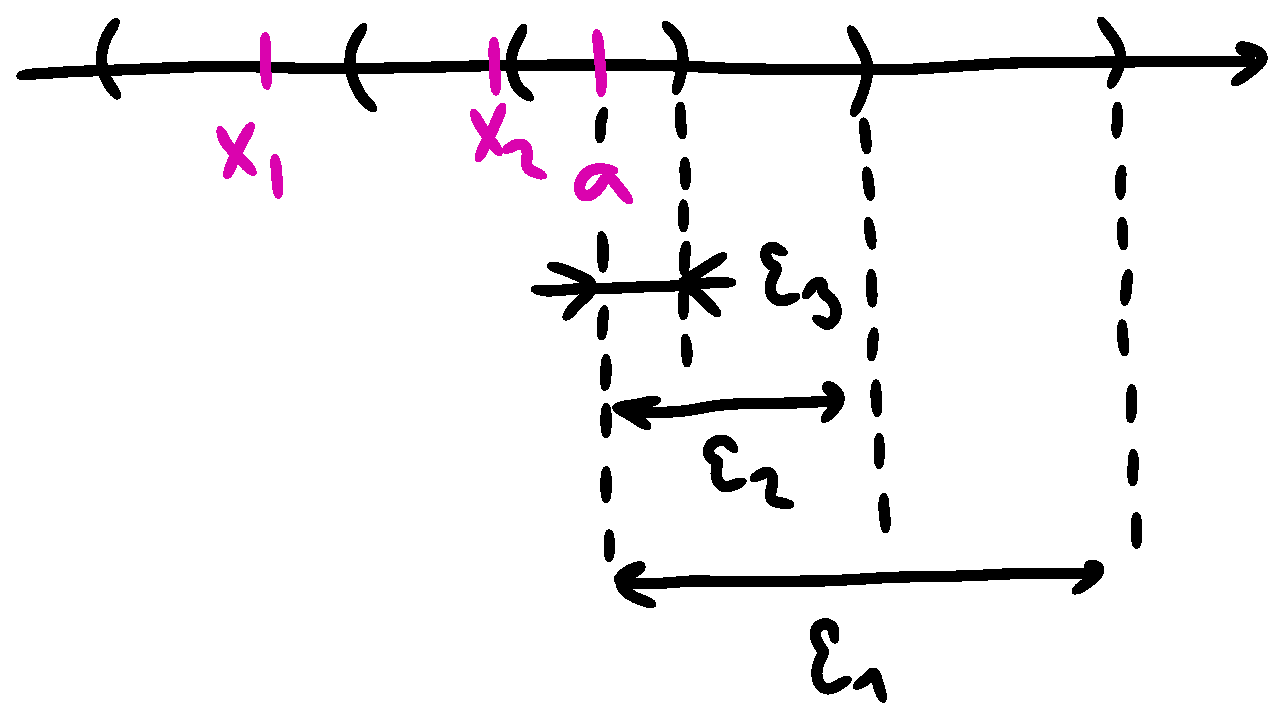
\includegraphics[width=0.6\linewidth]{images/xn-to-a}
      
      \caption{
        Если в любой $\eps$-окрестности~$a$ есть элемент последовательности, то можно построить сходящуюся к~$a$ подпоследовательность.
      }
      \label{fig:xn-to-a}
    \end{figure}
 
  \end{solution}
  
  
  \subsection{Просто номер 1 (``лемма-номер'' к следующему)}\label{sec:simple-no-1}
  
  Доказать, что
  \begin{equation}\label{eq:lemma-no}
    \lim_{n \to \infty} \frac{n}{a^n} = 0,\quad a > 1
  \end{equation}
  
  % https://math.stackexchange.com/a/55488/451127
  \begin{solution}
    Так как $a \hm> 1$, то можно положить:
    \[
      a = 1 + \alpha,\quad \alpha > 0
    \]
    
    Рассмотрим теперь отдельно знаменатель:
    \[
      a^n = (1 + \alpha)^n = \underbrace{(1 + \alpha) \cdot (1 + \alpha) \cdot \ldots \cdot (1 + \alpha)}_{n} = \blacktriangle
    \]
    
    Начнём перемножать скобки.
    Их ``много'', поэтому предложим алгоритм перемножения.
    Если из каждой выбрать слагаемое ${+}1$, то в результате получим просто $1^n \hm= 1$.
    Далее, из одной (какой-нибудь) скобки выберем~$\alpha$, а из всех других~$1$.
    Получим $\alpha \hm\cdot 1^{n - 1}$.
    Но сколько есть способов выбрать из~$n$ скобок ту, в из которой берём~$\alpha$?
    Очевидно, $n$ способов.
    Итого, в результате перемножения скобок получим такое слагаемое с~$\alpha$ в первой степени: $n \alpha$.
    Теперь выбираем $\alpha$ из двух скобок (из других берём~$1$).
    Способов выбрать две скобки из~$n$ всего есть~$C_n^2 \hm= \frac{n!}{2!\,(n - 2)!} \hm= \frac{n(n - 1)}{2}$.\footnote{
      В институтских курсах комбинаторики число сочетаний из $n$ по $k$ также обозначается как $\binom{n}{k} = C_n^k$.
    }
    Ограничимся этими слагаемыми (где $\alpha$ в степени до квадрата включительно:
    \[
      \blacktriangle = 1 + n \alpha + \frac{n(n - 1)}{2} \alpha^2 + \ldots
    \]
    
    Вернёмся к пределу~\eqref{eq:lemma-no}:
    \begin{equation*}
    \begin{split}
      \lim_{n \to \infty} \frac{n}{a^n}
        = \lim_{n \to \infty} \frac{n}{(1 + \alpha)^n}
        &= \lim_{n \to \infty} \frac{n}{1 + n \alpha + n(n - 1)/2 \cdot \alpha^2 + \ldots}\\
        &= \lim_{n \to \infty} \frac{1}{1/n + \alpha + (n - 1)/2 \cdot \alpha^2 + \ldots}
        = 0
    \end{split}
    \end{equation*}
    % TODO: some note or something (about lim 1/n^2)
  \end{solution}
  
  
  \subsection{С1, \S 8, \textnumero 64(3)}
  
  Найти $\lim\limits_{n \to \infty} x_n$:
  \[
    x_n = \sqrt[n]{3^n + n \cdot 2^n}
  \]
  
  \begin{solution}
    % Показать, что предел есть (или считать, что он есть, и если получится найти, то и есть)
    По-хорошему, перед тем, как считать предел, стоило бы сначала понять, точно ли последовательность сходится.
    Однако... можно просто попытаться найти предел, и если получится~---~то и хорошо (значит, сходится).
    
    Имея в виду номер~(\ref{sec:simple-no-1}), несложно догадаться, что надо сделать в этом ($3^n$ по корнем растёт быстрее, чем $n \hm\cdot 2^n$):
    \[
      \lim\limits_{n \to \infty} \sqrt[n]{3^n + n \cdot 2^n}
        = \lim\limits_{n \to \infty} \sqrt[n]{3^n \left(1 + \frac{n \cdot 2^n}{3^n}\right)}
        = \lim\limits_{n \to \infty} 3 \cdot \sqrt[n]{1 + \frac{n}{(3/2)^n}}
        = 3
    \]
    где в последнем переходе на самом деле также использовался тот факт, что
    \[
      \lim_{n \to \infty} \sqrt[n]{1 + \alpha_n} = 1\quad \mbox{при}\quad \lim_{n \to \infty} \alpha_n = 0
    \]
    
    Покажем также и это...
    Другими словами, надо показать, что:  % \footnote{Кроме как по определению, не очень понятно, что с этим делать...}
    \[
      \forall \eps > 0\ \exists N \in \NN\colon \forall n \geq N \to \left|\sqrt[n]{1 + \alpha_n} - 1\right| < \eps
    \]
    
    Рассмотрим отдельно неравенство:
    \[
      1 - \eps < \sqrt[n]{1 + \alpha_n} < 1 + \eps
    \]
    
    Возводя в $n$-ую степень все части (с левой, по-хорошему, опять надо быть осторожнее, потому что она в принципе может быть меньше нуля, однако сосредоточимся на основном):\footnote{
      Вообще, можно объяснить, что достаточно рассматривать лишь $\eps \in (0, 1]$, и в таком случае проблем со знаком левой части в неравенстве не будет.
    }
    \[
      (1 - \eps)^n < 1 + \alpha_n < (1 + \eps)^n = 1 + n \eps + \ldots
    \]
    
    Так как $\alpha_n$ бесконечно малая, то для используемого~$\eps$ найдётся~$N$, начиная с которого $\alpha_n \hm< \eps$, а потому и $\alpha_n \hm< n \eps$.
  \end{solution}
  
  \begin{remark}
    В информатике есть понятие \emph{сложности алгоримтов}.
    Сложность может быть пространственной (сколько памяти надо для работы программы) и временной (сколько ``атомарных'' операций надо выполнить в течение исполнения программы).
    Сложности оценивают как функции от параметров задачи.
    
    Например, пусть надо найти максимальный элемент среди $N$ элементов.
    Как это сделать?
    Надо просмотреть все элементы от первого до последнего, на каждом шаге помня максимальный элемент из увиденных ранее.
    Пространственная сложность складывается из хранения массива, плюс числа~---~максимального элемента (или номера по списку элемента, который максимальный).
    Итого~---~\emph{примерно} $N$ чисел.
    Временн\'{а}я сложность складывается из просмотра всех элементов (сравнений каждого элемента с текущим максимальным).
    Итого~---~тоже \emph{примерно} $N$ операций.
    Сложности оцениваются не с точностью до одной операции/числа, которое надо хранить.
    Как правило, интересна \emph{асимптотика}~---~поведение оценки сложности при больших~$N$.
    
    Другой пример: сортировка массива.
    Рассмотрим такой:
    \[
      [2, 3, 1, 5, 4]
    \]
    Отсортировать массив~---~значит расположить его элементы по возрастанию.
    Как это сделать?
    Предлагается такой алгоритм: искать минимальный, ставить его в начало (переставлять местами с первым), искать минимальный среди оставшихся, ставить его на второе место (переставлять местами со вторым), и так далее до конца.
    Процесс сортировки приведённого массива по такому алгоритму будет выглядеть так (цветом выделена уже отсортированная часть):
    \[
      \begin{aligned}
        &[2, 3, 1, 5, 4]\\
        &[\textcolor{pink}{1}, 3, 2, 5, 4]\\
        &[\textcolor{pink}{1, 2}, 3, 5, 4]\\
        &[\textcolor{pink}{1, 2, 3}, 5, 4]\\
        &[\textcolor{pink}{1, 2, 3, 4}, 5]\\
        &[\textcolor{pink}{1, 2, 3, 4, 5}]\\
      \end{aligned}
    \]
    Итого процесс занял несколько итераций, на каждой из которых было проведено столько-то сравнений.
    Посчитаем общее количество сравнений (по сути это количество элементов ``не в цвете'' на каждой итерации):
    \[
      5 + 4 + 3 + 2 + 1 = 15
    \]
    
    В общем случае (при размере массива~$N$) операций будет совершено:
    \[
      N + (N - 1) + \ldots + 2 + 1 = \frac{N(N + 1)}{2} \sim N^2
    \]
    то есть при больших~$N$ сложность сравнима с~$N^2$.
    
    Часто встречаемые на практике асимптотики временн\'{о}й сложности представлены на картинке~(\ref{fig:complexities}).
    
    % TODO: refine picture (colors + sqrt n), or make a new one; png -> svg
    \begin{figure}[ht]
      \centering
      \includegraphics[width=0.8\linewidth]{images/Comparison_computational_complexity}
      
      \caption{
        ``Популярные'' (кроме, возможно, корня и факториала) асимптотики временн\'{о}й сложности алгоритмов.
        ({\small Источник: \href{https://it.wikipedia.org/wiki/File:Comparison\_computational\_complexity.svg}{it.wikipedia.org/wiki/File:Comparison\_computational\_complexity.svg}.})
      }
      \label{fig:complexities}
    \end{figure}
  \end{remark}
  
  \subsection{Просто номер 2 (вдогонку к предыдущему)}
  
  Доказать, что
  \[
    \lim_{n \to \infty} \frac{\log_2 n}{n} = 0
  \]
  
  % https://math.stackexchange.com/a/1723885/451127
  \begin{solution}
    % TODO: график
    % Графический способ
    
    Если вспомнить графики функций $y \hm= \log_2 n$ и $y \hm= n$, то становится понятно, почему предел нулевой: первая растёт намного медленнее, чем вторая.
    Однако... такой ``графический способ'', хоть и быстрый и наглядный, но недостаточно ``строгий''~---~по-хорошему, надо бы было всё-таки строго показать, что отношение $\frac{\log_2 n}{n}$ начиная с какого-то~$N$ становится больше любого наперёд заданного~$C \hm> 0$...
    
    Поэтому сделаем по-другому.
    Имея $\{x_n\}$, построим новую последовательность $\{y_n\}$, такую что:
    \[
      y_n = 2^{x_n} = \sqrt[n]{n}
    \]
    Если $x_n \hm{\xrightarrow{n \to \infty}} 0$, то при этом, очевидно, будет $y_n \hm= 2^{x_n} \hm{\xrightarrow{n \to \infty}} 1$.
    Будет верно и наоборот: если покажем, что $y_n \hm{\xrightarrow{n \to \infty}} 1$, то это будет означать $x_n \hm= \log_2 y_n \hm{\xrightarrow{n \to \infty}} 0$.
    (Примем это как данность~---~или лучше оставим доказательство этого утверждения ``в качестве упражнения''.)
    
    Потому рассмотрим неравенство:
    \[
      1 - \eps < \sqrt[n]{n} < 1 + \eps
    \]
    
    Возводя в степень (посмотрим только на правую часть):
    \[
      n < (1 + \eps)^n = 1 + n \eps + \frac{n(n - 1)}{2} \eps + \ldots
    \]
    
    Начиная с какого номера~$N$ будет истинно это неравенство?
    При больших~$n$: $n \hm> 1$, $n \hm> n \eps$...
    Но посмотрим на третье слагаемое справа:
    \[
      \frac{n(n - 1)}{2} \eps = n \cdot \frac{n - 1}{2} \eps
    \]
    Если $\frac{n - 1}{2} \eps \hm> 1$, то это слагаемое одно окажется больше~$n$ (который стоит в левой части неравенства выше):
    \[
      \frac{n - 1}{2} \eps > 1 \leftrightarrow n > \frac{2}{\eps} + 1
    \]
    
    И потому в качестве номера~$N$ можно положить:
    \[
      N = \left\lceil\frac{2}{\eps}\right\rceil + 2
    \]
    
    Получили $y_n \hm= 2^{x_n} \hm{\xrightarrow{n \to \infty}} 1$, откуда $x_n \hm{\xrightarrow{n \to \infty}} 0$.
  \end{solution}
  
  
  %%% TODO (next time)
  
  %\subsection{С1, \S 8, \textnumero 143(1)}
  %
  %Доказать, что последовательность~$\{x_n\}$ сходится:
  %\[
    %x_n = \frac{\sin a}{2} + \frac{\sin{2a}}{2^2} + \ldots + \frac{\sin{na}}{a^n},\quad a \in \RR
  %\]
  %
  %\begin{solution}
    %% Два способа: просто и через Коши
  %\end{solution}
  %
  %
  %\subsection{С1, \S 8, \textnumero 158}
  %
  %Привести пример расходящейся последовательности~$\{x_n\}$, такой что
  %\[
    %\lim_{n \to \infty} |x_{n + p} - x_{n}| = 0,\quad \forall p \in \NN
  %\]
  %\begin{solution}
  %\end{solution}
  %
  %
  %\subsection{С1, \S 8, \textnumero 91}
  %
  %Верны ли утверждения?
  %\begin{enumerate}
    %\item Всякая бесконечно большая последовательность неограничена.  % TODO: неограничена или неограниченна
    %\item Всякая неограниченная последовательность является бесконечно большой.
  %\end{enumerate}
  %
  %\begin{solution}
  %\end{solution}
  %
  %
  %\subsection{С1, \S 8, \textnumero 119}
  %
  %Доказать, что последовательность сходится тогда и только тогда, когда она ограничена и имеет один (и только один) частичный предел.  % TODO: ограничена или ограниченна
  %
  %\begin{solution}
  %\end{solution}
  %
  %
  %\subsection{С1, \S 8, \textnumero 120}
  %
  %У последовательности $\{x_n\}$ подпоследовательности $\{x_{2k}\}$, $\{x_{2k - 1}\}$ и $\{x_{3k}\}$ сходятся.
  %Доказать, что сходится и сама последовательность.
  %
  %\begin{solution}
  %\end{solution}
  
\end{document}
